
\chapter{REFERENCIAL TEÓRICO}
\label{chap:ref_teo}

% Neste capítulo serão apresentadas as ferramentas que serão utilizadas no decorrer do presente trabalho, bem como, o conceito básico de cada uma. 

Durante o desenvolvimento do projeto, o programador deve estar ciente de quais técnicas deverão ser aplicadas. A primeira delas é saber qual é o público alvo que aquela aplicação terá, a segunda é entender qual será a abordagem do desenvolvimento, podendo assim ter esclarecido para quais plataformas o aplicativo poderá ser executado, o projeto pode ser destinado ao Android, ao iOs, ou para as duas ao mesmo tempo.

\citeonline{apps} fala em seu artigo que existem três abordagens básicas quanto à forma de desenvolvimento de aplicativos, cada uma com suas potencialidades, restrições e cuidados especiais. As técnicas são as seguintes: desenvolvimento nativo, desenvolvimento web e desenvolvimento híbrido.

\section{Aplicativo Nativo}

Um aplicativo nativo é focado em uma plataforma ou conjunto de dispositivos específicos e desenvolvido pelo modelo de programação desta plataforma. Ele pode utilizar todos os recursos do telefone, como geolocalização, câmera, aplicativos de mídia, notificações entre outros. Os aplicativos nativos são escritos na linguagem de programação específica de cada sistema operacional, sendo as mais populares \textit{Swift} para aparelhos Apple e Java para aparelhos Android. \cite{apps}

Aplicativos nativos geralmente são escolhidos como metodologia de desenvolvimento pois conseguem ter um desempenho superior e por utilizar melhor os recursos do hardware que os aplicativos híbridos e os \textit{Web App}.


\section{Aplicativo Web}
As \textit{Progressive Web Apps} (PWA) são aplicações que podem ser acessadas através do navegador, tanto do celular quanto do computador ou tablet, já que ele é basicamente um site, onde pode ser executado no dispositivo móvel por meio da reponsividade. São desenvolvidos em \textit{HTML, CSS} e \textit{JavaScript}, podem ser acessados através de uma \textit{URL} e reduzem bastante o tempo de desenvolvimento, se for comparado a um aplicativo híbrido, pois o código desta aplicação será reaproveitado para executar em outra plataforma. \cite{apps}


% Basicamente as PWA 

\section{Aplicativo Híbrido}
As aplicações híbridas são resultados da execução de um único projeto, funcionando normalmente em mais de um sistema operacional simultaneamente. Isso significa que, ao criar um aplicativo que executa em um aparelho com sistema operacional Android, ele pode também funcionar em um aplicativo com sistema operacional iOs e, com isto, o tempo e custo de desenvolvimento acabam sendo reduzidos. Não é considerado uma aplicaçao que tem fácil acesso aos recursos do telefone. Também possui desempenho inferior ao aplicativo nativo. \cite{apps}

A mão de obra acaba sendo mais cara para programadores que desenvolvem para uma única plataforma e, por este motivo, diversas empresas pensam bastante antes de dar início a construção de algo que irá tomar mais tempo e terá um custo maior, já que terão que desenvolver dois projetos simultaneamente. Muitas dessas empresas acabam obtando por desenvolver uma única aplicação que possa abranger as duas plataformas, que também será o caso do desenvolvimendo deste trabalho. 

\citeonline{appnativo} ressalta três principais características sobre os apps. Os aplicativos nativos possuem melhor usabilidade, pois o desempenho e performance dessas aplicações geralmente são melhores, a maioria deles podem ser acessados offline. Os PWAs geralmente são utilizados em cenários em que não haja tanta interação com os consumidores e ainda, eles não conseguem utilizar todos os recursos que o smartphone disponibiliza.

% \subsection{Banco de Dados Relacional}

% \subsection{Banco de Dados Não Relacional}

% \chapter{FERRAMENTAS DE DESENVOLVIMENTO FRONT-END}

\section{React Native}

O \textit{React Native} é um projeto \textit{open-source} desenvolvido por engenheiros do Facebook e mantido por uma grande comunidade de voluntários, através do \textit{GitHub}. Este \textit{framework} é escrito utilizando a linguagem \textit{JavaScript} que é a linguagem mais utilizada do mundo e também, o \textit{JavaScript} é uma linguagem de comportamento que permite a criação de conteúdos dinâmicos, é considerada uma linguagem de alto-nível, padronizada, utilizada para desenvolvimento de projetos complexos, permite a criação de conteúdos dinâmico, agindo com facilidade em testar o próprio código de forma rápida. \cite{javascript}

O RN utiliza chamadas nativas para que os elementos possam sem renderizados afim de representar os elementos da interface do usuário. Para fazer a renderização desses elementos o \textit{React Native} utiliza um conceito chamando de \textit{Bridge}, e é o que diferencia o \textit{framework}, esta serve para a comunicação do nativo com o \textit{JavaScript}.

\cite{rn} ressalta que existem três \textit{threads} principais que são executadas em uma aplicação utilizando o \textit{framework} React Native, onde uma é utilizada para tratar as requisições relacionadas a renderização de elementos na tela e também pelos gestos reproduzidos pelo usuário, a outra é exclusiva ao React Native, que é responsável por executar o código JavaScript. O JavaScript é o responsável por toda lógica de negócio da aplicação. Além de definir a estrutura e as funcionalidades da interface do usuário. E por último, existe aquela que é a responsável pelos cálculos referentes ao layout. 


Ao utilizar a ferramenta \textit{React Native} para a construção de um aplicativo móvel, tem-se o desenvolvimento de um aplicativo considerado nativo na qual, é possível acessar diversos recursos do próprio dispositivo, e mesmo assim manter um único código fonte funcional para mais de uma plataforma simultaneamente e sem perder desempenho por isso. Neste caso de uso será utilizado as plataformas Android e iOS para fazer a compilação dos aplicativos.
\citeonline{reactNative} diz que o \textit{React Native} é \textit{JavaScript} rodando em uma máquina virtual e controlando a interface do usuário nativa.

% \citeonline{javascript}, descreve o \textit{JavaScript} como sendo a linguagem mais utilizada do mundo, é uma linguagem de comportamento que permite fazer a criação de conteúdos dinâmicos, entre outros. Consiste em ser uma linguagem de alto-nível, padronizada, é uma ferramenta para desenvolvimento de projetos complexos e também age com facilidade em testar o próprio código de forma muito rápida. Com \textit{JavaScript} é que o \textit{React Native} é escrito.


\section{JSX}
O \textit{JSX} é uma extensão de sintaxe para \textit{JavaScript}, recomendada para auxílio na construção da interface gráfica que será utilizada com o \textit{React} e, também, com o \textit{React Native}, para falicitar a estrutura de códigos durante o desenvolvimento do \textit{front-end}. Ele necessita de um tradutor, ou seja, de uma ferramenta que possa traduzir o código em algo que o JavaScript conheça e a ferramenta mais utilizada para fazer este processo é o \textit{Babel}. Possui uma sintaxe muito semelhante à do \textit{XML}.  
\cite{jsx}.


\section{ReactJS}
\textit{ReactJS} se diferencia de \textit{React Native} por ser uma plataforma voltada para aplicações web. É uma biblioteca JavaScript. Também é uma tecnologia considerada nova, hoje grandes empresas também fazem o uso do \textit{ReactJS}, como é o caso do Facebook, Netflix, AirBnB, Instagram entre outros. Também pode ser utilizado \textit{JSX} pra facilitar na estrutura da interface do usuário e é uma tecnologia nova que está crescendo cada dia mais, também foi criada pelos engenheiros do Facebook e inclusive, esta biblioteca é \textit{open source} e mantida por comunidades do \textit{GitHub}, na qual fazem com que melhorias constantes sejam realizadas, suprindo cada vez mais a necessidade dos desenvolvedores. \cite{react}

A escolha da utilização do \textit{ReactJS} para codificar a aplicação web, se deu devido a facilidade de utilização, já que pode ser considerado um framework fracamente acoplado. Utiliza-se componentização que faz com que haja reaproveitamento de código em outras partes do projeto, tornando assim o desenvolvimento mais padronizado, simples e limpo.

\section{Ecmascript}

\textit{Ecmascript} é a especificação da linguagem de script que o JavaScript implementa. É padronizada pela empresa Ecma International, e por isto leva este nome, já que faz a união da nomenclatura da empresa com a palavra script. 

Em 2015, foi lançada uma atualização que teve muitas melhorias, dentre elas: simplificação de sintaxe, nova forma de declarar as variáveis, entre outros \cite{ecma}.
Foi através das evoluções do ESCAScript2, ou ainda, \textit{ES6} e \textit{ES2015} como também pode ser chamado, que a comunidade se sentiu motivada em utilizar bibliotecas e frameworks, como \textit{React} e \textit{React Native}. 

% \chapter{FERRAMENTAS DE DESENVOLVIMENTO BACK-END}

\section{NodeJS}
NodeJS é uma plataforma JavaScript que executa no lado do servidor, possibilitando a construção de aplicações escaláveis e de baixa latência. Com ele é possível construir uma aplicação servidor incrivelmente rápida para atender milhares de requisições concorrentes com um \textit{overhead} mínimo e utilizando um único processo. Sendo um processo de thread única, o consumo de memória é muito baixo em relação a servidores de aplicações atuais, além de ser uma aplicação sem bloqueios de execução. \cite{node}

Apesar da ideia original ser essa, Node não é só um servidor. É é possível que sejam montados servidores \textit{http} e  \textit{https}, assim como servidores de  \textit{DNS, TCP, Media Server} e etc. Agora também é possível criar aplicações desktop com o  \textit{Node-WebKit} e até mesmo ambientes de desenvolvimento para front-end. \cite{node1}


% Várias outras atividades podem ter sido executadas pelo loop do Node sem ter interrompido o funcionamento ou bloqueado a thread, já que o node possui um loop infinito que executa ações de eventos em um pilha de eventos, as atividades desses eventos sao processadas de maneira assíncrona pelas bibliotecas internas desenvolvidas em C e C++, tendo como resultado dessas chamadas o retorno quando o trabalho em questão estiver concluído.

O desevolvimento da comunicação dos dados através de uma \textit{API} (Application Progress Interface) é feito em JavaScript,  e o líder de soluções \textit{open source} \citeonline{api}, diz que uma \textit{API} é uma interface de programação de aplicações, onde permite integrar \textit{API}'s de outros softwares, podendo assim, realizar a comunicação entre eles. Com este conceito definido, será realizada a integração do \textit{back-end} com a aplicação \textit{front-end} da web e será feita a comunicação entre elas, juntamente com a comunicação do aplicativo, na qual os registros serão lançados no app mobile e, através de uma sincronização de dados, será feito o envio das informações para o servidor da \textit{API}, permitindo que os usuários façam a consulta dos dados na página disponível na web.

\section{NestJS}
O \textit{NestJS} foi escolhido dentre as tecnologias para o desenvolvimento proposto, pois entende-se que pode diminuir a ocorrência de erros em tempo de execução, já que o servidor NestJS é compilado sobre um servidor Node.JS. Esta ferramenta se diferencia na oferta de arquitetura de aplicativos pronta para a criação de aplicativos altamente testáveis, escalonáveis e de fácil manutenção.

Ele é extensivo, pois fornece uma verdadeira flexibilidade, permitindo o uso de outras bibliotecas graças à arquitetura modular, organizando o código em módulos separados. Possui um ecossistema adaptável que é um \textit{backbone} completo para todos os tipos de aplicativos do lado do servidor. Aproveita os recursos mais recentes do JavaScript, trazendo padrões de design e soluções maduras para o mundo node.js, tornado-se assim progressivo. \cite{nest}

\section{Firebase}
Segundo \citeonline{firebase}, o Firebase é um Baas (\textit{Backend as a Service}) para aplicações web e mobile do Google. Foi lançado em 2004 e, com o passar dos anos, cresceu muito. Com este serviço é possível integrar \textit{push notification}, realizar configurações de servidor e também fazer a integração com banco de dados além de outros.

O Firebase utiliza banco de dados hospedado na nuvem chamado de Firebase Realtime Database. Os dados são armazenados como JSON e sincronizados em tempo real com todos os clientes conectados. Quando são criadas aplicações em plataformas utilizando SDKs para iOS, Android e JavaScript, todos os clientes compartilham uma instância do Realtime Database e recebem automaticamente atualizações com os dados mais recentes.  \cite{firebase1} 

\section{Tecnologias já existentes}
Várias \textit{startups} do Brasil estão criando soluções inovadoras na área do agronegócio. Com o intuito de gerar bons resultados com essas soluções, grandes empresas investem em eventos deste tipo, para que a inovação seja promovida e que novas ideias sejam desenvolvidas.

Um desses eventos contou com a participação da equipe Gravitwave \footnote {Startup brasileira Catarinense que atua com soluções inovadoras no agronegócio, https://gravitwave.com/}, que se destacou com um WebApp para o gerenciamento da criação de porcos a Coopig, e também com outra aplicação para o controle de frangos de corte, chamada Cocoriko. A última citada, conta com a ajuda do produtor rural, para fazer o controle dos gastos e também conduzir o preenchimento da coleta diária das informações de cada aviário.

\begin{figure}[!h]
    \centering
    \caption{Tela de login, do aplicativo Cocoriko}
    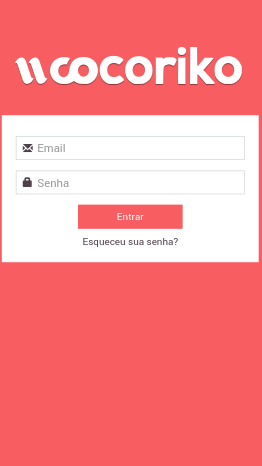
\includegraphics[width=0.3\textwidth]{./dados/figuras/cocoriko.png}
    \fonte{Autor}
    \label{fig:p1}
\end{figure}

Uma outra startup que também tem o foco voltado para a agroindústria de aves, é a Stac\footnote{Startup Paranaense que investiu em ferramenta para ajudar o dia a dia do avicultor, https://agrostac.com.br/}. Eles possuem um \textit{hardware} com sensores para captar informações internas dos aviários e um aplicativo chamado AveStac mais focado para a conversão alimentar dos frangos. Conversão esta que é muito importante para gerar lucros no negócio. Além de ter poder fazer o manejo e o planejamento das atividades desenvolvidas pelo avicultor.                                                          \begin{figure}[h]
    \centering
    \caption{Telas do aplicativo Avestac}
    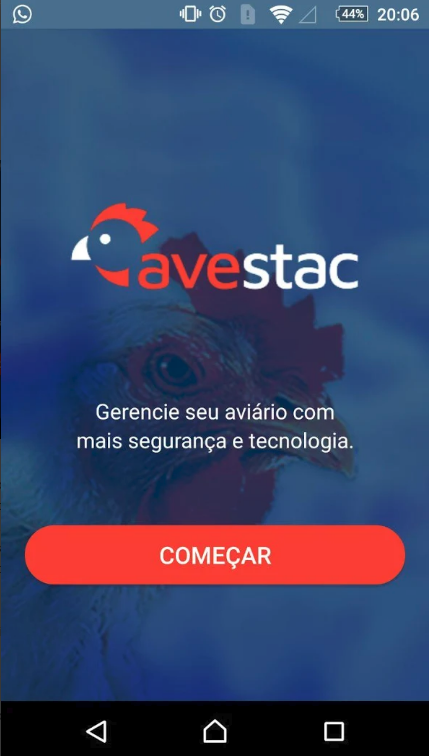
\includegraphics[width=0.3\textwidth]{./dados/figuras/avestac1.png}
    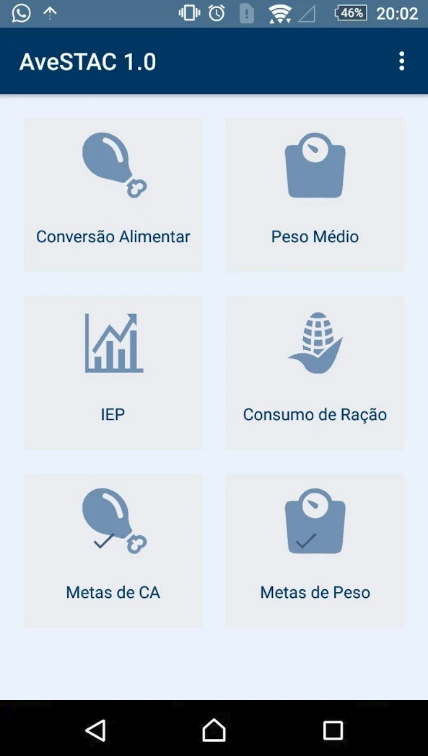
\includegraphics[width=0.3\textwidth]{./dados/figuras/avestac2.png}
    \fonte{Autor}
    \label{fig:p1}
\end{figure}                                                                       

% ********** Tabelas exemplo Diagrama Caso de Uso ********** %

% \begin{table}[H]
% \centering
% \begin{tabular}{|l|l|} 
% \hline
% Caso de Uso:   & Realizar cadastro                       \\ 
% \hline
% Ator(es):      & Usuário                                 \\ 
% \hline
% Pré-condições: & Usuário não pode ter tido acesso antes  \\ 
% \hline
% Pós-condições: & Cadastro realizado e login efetuado     \\
% \hline
% \end{tabular}
% \end{table}

% \begin{table}[H]
% \centering
% \begin{tabular}{|l|l|l|l|l|} 
% \hline
%  & Ator                          &  & Sistema &   \\ 
% \hline
% 1 & Usuário precisa realizar login no aplicativo                           &  &         &   \\ 
% \hline
%  &                               & 2 & O sistema mostra por onde você pode realizar o login        &   \\ 
% \hline
% 3 & Usuário acessa o aplicativo e
% precisa realizar login                              &  &         &   \\ 
% \hline
%  &                               &  &         &   \\ 
% \hline
%  &                               &  &         &   \\ 
% \hline
%  &                               &  &         &   \\ 
% \hline
%  &                               &  &         &   \\
% \hline
% \end{tabular}
% \end{table}

% \begin{table}[H]
% \centering
% \begin{tabular}{|l|l|} 
% \hline
%   &   \\ 
% \hline
%   &   \\ 
% \hline
% ~ &   \\ 
% \hline
%   &   \\
% \hline
% \end{tabular}
% \end{table}